The following sections provide system and component level performance results of the implemented PLL based from parasitic extracted transistor level simulations of the design.
\subsection{Power Breakdown}
\vspace{-1em}
\FloatBarrier
\begin{figure}[htb!]
	\begin{floatrow}
	\ffigbox{%
		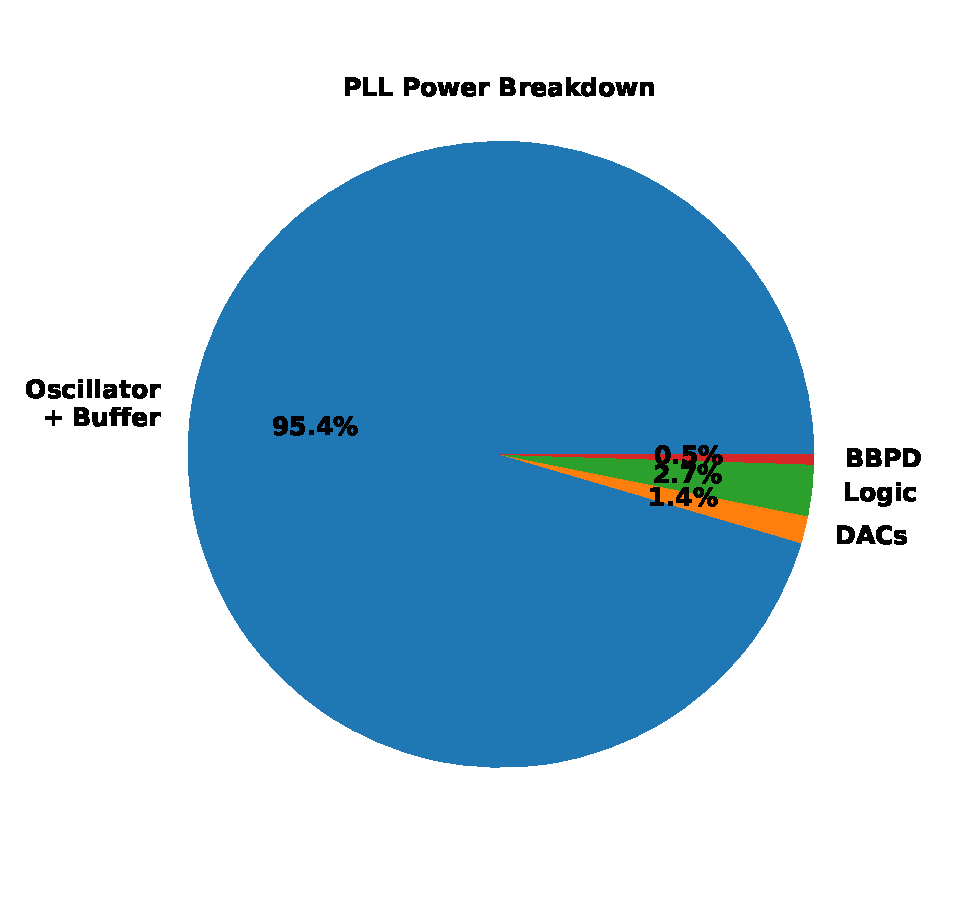
\includegraphics[width=0.5\textwidth, angle=0]{./figs/results/power_bkdn}
	}{%
		\caption{PLL Power breakdown.}
		\label{fig:pow_bkdn}
	}
	\capbtabbox{%
		\def\arraystretch{1.5}		
		\setlength\arrayrulewidth{0.75pt}
		\setlength{\tabcolsep}{1em} % for the horizontal padding
			\begin{tabular}{|c|c|c|}
				\hline 
				\rule[-1ex]{0pt}{2.5ex} \cellcolor{gray!40}\textbf{Component} & \cellcolor{gray!40}\textbf{Power [$\mu$W]} & \cellcolor{gray!40}\textbf{\% of Total}\\ 
				\hline 
				\rule[-1ex]{0pt}{2.5ex} \textbf{VCO + Buffer} &  90.62 & 95.4 \\ 
				\hline 
				\rule[-1ex]{0pt}{2.5ex} \textbf{2x 3b CDAC} & 0.071 &  $<$ 0.01  \\ 
				\hline 
				\rule[-1ex]{0pt}{2.5ex} \textbf{2x 10b CDAC} &  1.33 &  1.40  \\ 
				\hline 
				\rule[-1ex]{0pt}{2.5ex} \textbf{BBPD} &  0.462 &  0.49  \\ 
				\hline 
				\rule[-1ex]{0pt}{2.5ex} \textbf{Logic} &  2.51 &  2.64  \\ 
				\hline 
				\rule[-1ex]{0pt}{2.5ex} \textbf{Total} &  95.0 &  100  \\ 
				\hline 
			\end{tabular} 
	}{%
		\caption{Power breakdown.}
		\label{tab:power_bkdn}
	}
	\end{floatrow}
\end{figure}		
{\color{white}.}
\FloatBarrier
\vspace{-3em}
\subsection{Area Breakdown}
\vspace{-1em}
\begin{figure}[htb!]
	\begin{floatrow}
	\ffigbox{%
		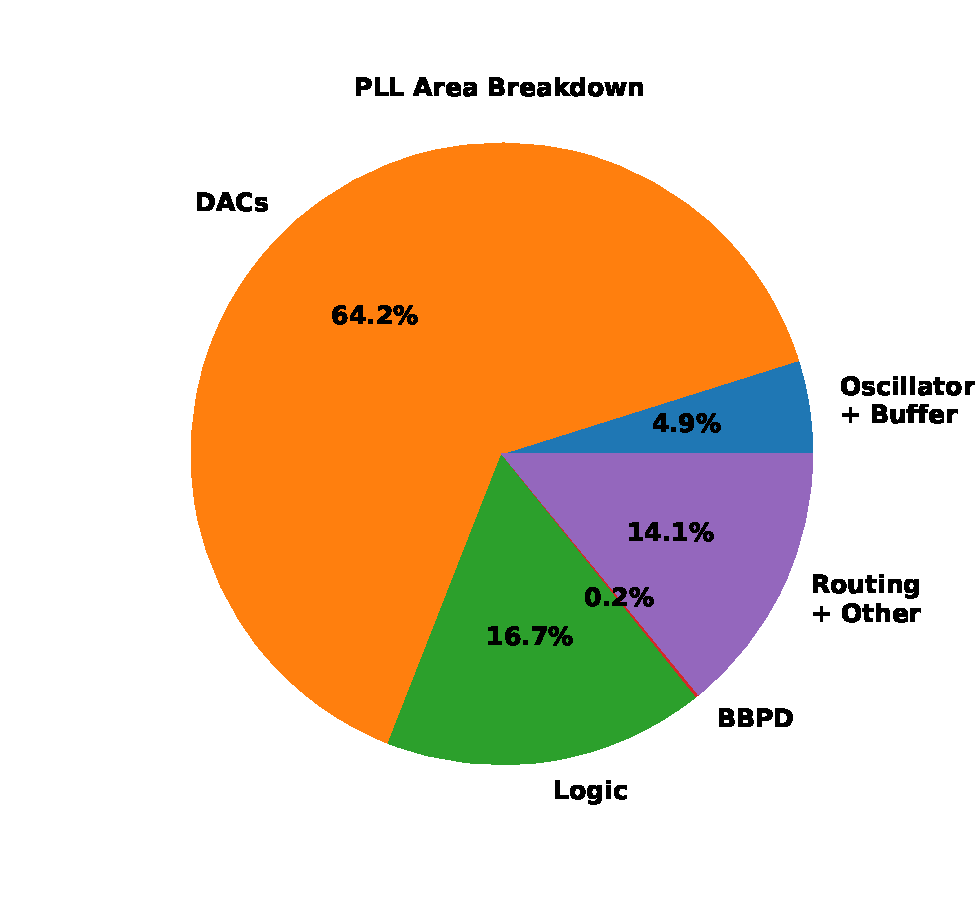
\includegraphics[width=0.5\textwidth, angle=0]{./figs/results/area_bkdn}
	}{%
		\caption{PLL Area breakdown.}
		\label{fig:area_bkdn}
	}
	\capbtabbox{%
		\def\arraystretch{1.5}		
		\setlength\arrayrulewidth{0.75pt}
		\setlength{\tabcolsep}{1em} % for the horizontal padding
			\begin{tabular}{|c|c|c|}
				\hline 
				\rule[-1ex]{0pt}{2.5ex} \cellcolor{gray!40}\textbf{Component} & \cellcolor{gray!40}\textbf{Area [$\mu$m$^2$]} & \cellcolor{gray!40}\textbf{\% of Total}\\ 
				\hline 
				\rule[-1ex]{0pt}{2.5ex} \textbf{VCO + Buffer} &  177.1 & 4.85 \\ 
				\hline 
				\rule[-1ex]{0pt}{2.5ex} \textbf{2x 3b CDAC} &  735.0 &  20.14 \\ 
				\hline 
				\rule[-1ex]{0pt}{2.5ex} \textbf{2x 10b CDAC} &  1607.7 &  44.05  \\ 
				\hline 
				\rule[-1ex]{0pt}{2.5ex} \textbf{BBPD} &  5.31 &  0.15  \\ 
				\hline 
				\rule[-1ex]{0pt}{2.5ex} \textbf{Logic} &  610.2 &  16.72  \\ 
				\hline 
				\rule[-1ex]{0pt}{2.5ex} \textbf{Other/routing} &  514.7 &  14.10  \\ 
				\hline 
				\rule[-1ex]{0pt}{2.5ex} \textbf{Total} &  3650 &  100  \\ 
				\hline 
			\end{tabular} 
	}{%
		\caption{Area breakdown.}
		\label{tab:area_bkdn}
	}
	\end{floatrow}
\end{figure}	

{\color{white}.}
\FloatBarrier


\subsection{PLL Phase Noise}

	\begin{figure}[htb!]
	    \centering
	    \begin{subfigure}{0.5\textwidth}
	        \centering
	        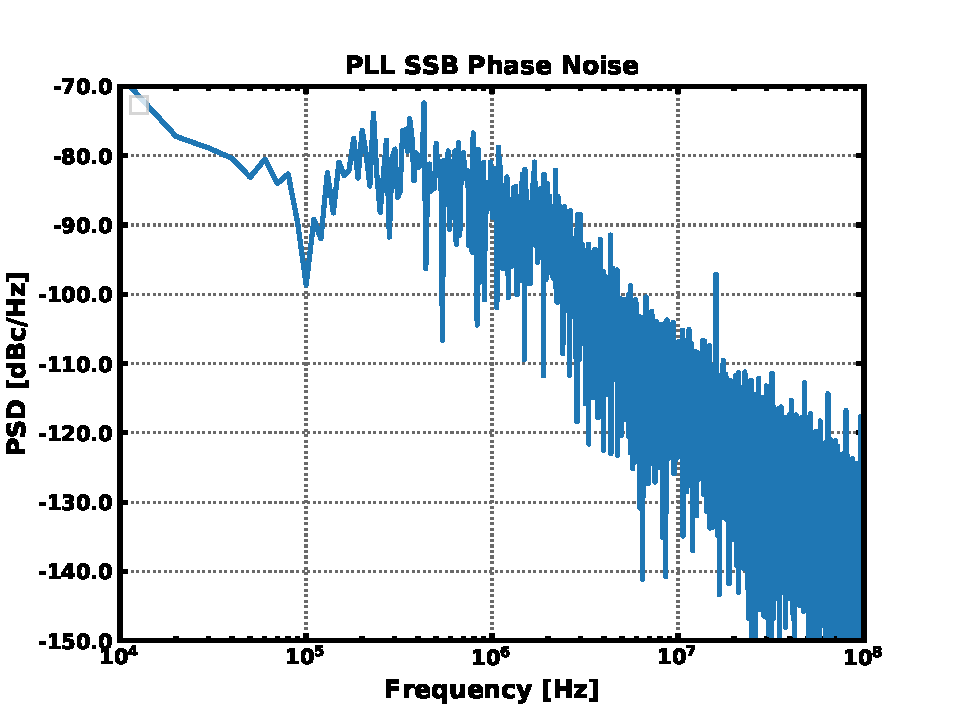
\includegraphics[width=1\textwidth, angle=0]{./figs/results/pll_pn_final_100u}
	        \caption{ }
	        \label{fig:sim_pll_psd}
	    \end{subfigure}%
	    \begin{subfigure}{0.5\textwidth}
	        \centering
	        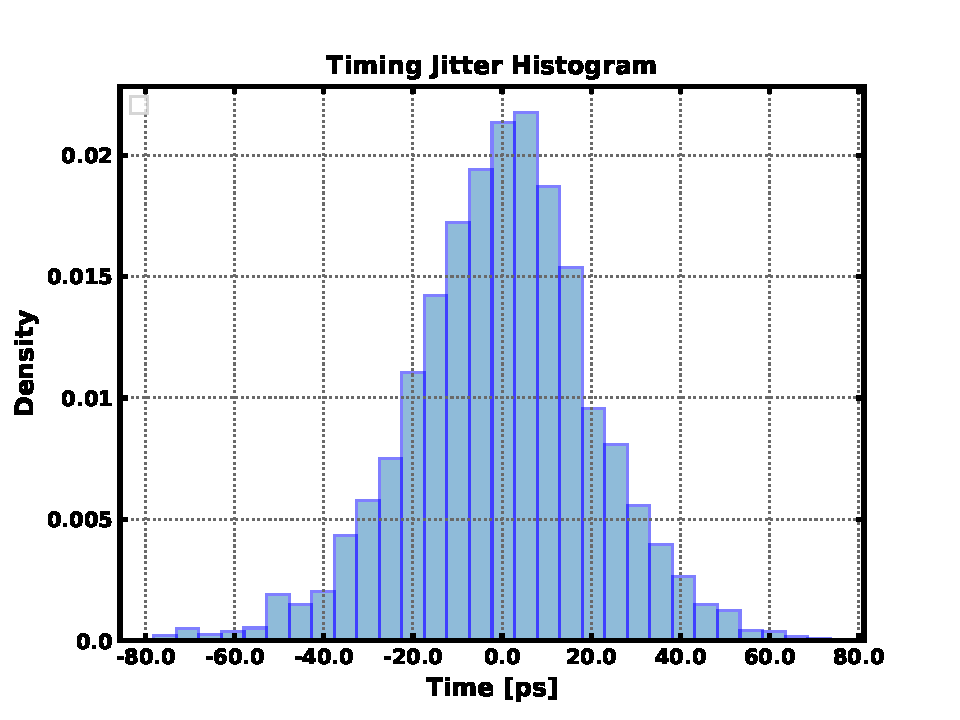
\includegraphics[width=1\textwidth, angle=0]{./figs/results/jitter_hist}
	        \caption{ }
	        \label{fig:pll_jit_hist}
	    \end{subfigure}
	    % \caption{x.}
	    \caption{\textbf{(a)} PLL phase noise SSB spectral density, \textbf{(b)} PLL jitter histogram.}
	    \label{fig:pll_pn_jit}
	\end{figure} 

\begin{table}[htb!]
	\def\arraystretch{1.5}		
	\setlength\arrayrulewidth{0.75pt}
	\setlength{\tabcolsep}{1em} % for the horizontal padding
	\begin{tabular}{|c|c|c|}
		\hline 
		\rule[-1ex]{0pt}{2.5ex} \cellcolor{gray!40}\textbf{Parameter} & \cellcolor{gray!40}\textbf{Value} & \cellcolor{gray!40}\textbf{Units}\\ 
		\hline 
		\rule[-1ex]{0pt}{2.5ex} \textbf{RMS Integrated Jitter} \tablefootnote{Up to 100 MHz}& 18.4 & ps \\ 
		\hline 
		% \rule[-1ex]{0pt}{2.5ex} $S_{0_{osc}}$ &  11885 &  rad$^2$/Hz  \\ 
		% \hline 
		\rule[-1ex]{0pt}{2.5ex} \textbf{FOM$_\textnormal{\textbf{jitter}}$} &  -224.9 & dB  \\ 
		\hline 
	\end{tabular} 
			\caption{PLL phase noise and jitter performance values.}
			\label{tab:pll_pn_jit_vals}
\end{table}




% \subsection{Start-up Transient}
% 	\hl{Lock time value.}
% 		\begin{figure}[htb!]
% 	        \centering
% 	        \includegraphics[width=0.65\textwidth, angle=0]{example-image}
% 		    \caption{PLL start up transient.}
% 		    \label{fig:sim_pll_trans}
% 		\end{figure}
% {\color{white}.}

\FloatBarrier
\subsection{Voltage Controlled Oscillator}\label{sec:ro_results}


	\subsubsection{Oscillator Phase Noise}
		\begin{figure}[htb!]
			\begin{floatrow}
			\ffigbox{%
				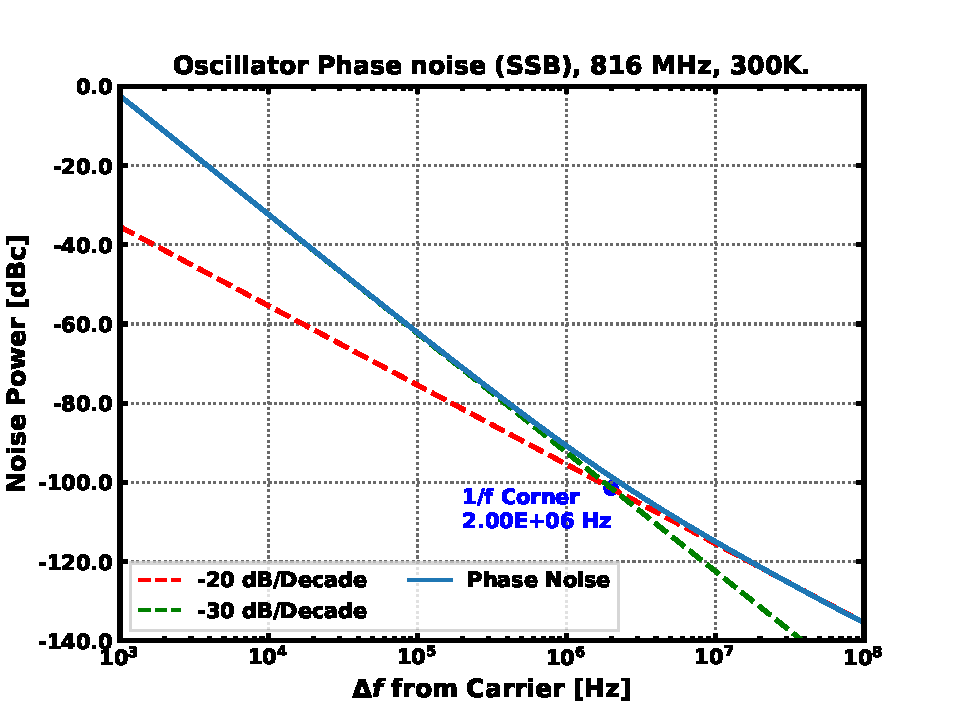
\includegraphics[width=0.55\textwidth, angle=0]{./figs/results/ro_pn_flicker}
			}{%
			    \caption{Ring oscillator phase noise (SSB).}
			    \label{fig:ro_pnoise}
			}
			\capbtabbox{%
				\def\arraystretch{1.5}		
				\setlength\arrayrulewidth{0.75pt}
				\setlength{\tabcolsep}{1em} % for the horizontal padding
				\begin{tabular}{|c|c|c|}
					\hline 
					\rule[-1ex]{0pt}{2.5ex} \cellcolor{gray!40}\textbf{Parameter} & \cellcolor{gray!40}\textbf{Value} & \cellcolor{gray!40}\textbf{Units}\\ 
					\hline 
					\rule[-1ex]{0pt}{2.5ex} \textbf{FOM$_{pn}$} & -158.9 & dB  \\ 
					\hline 
					% \rule[-1ex]{0pt}{2.5ex} $S_{0_{osc}}$ &  11885 &  rad$^2$/Hz  \\ 
					% \hline 
					\rule[-1ex]{0pt}{2.5ex} \textbf{Flicker corner} &  2.00 & MHz  \\ 
					\hline 
				\end{tabular} 
			}{%
				\caption{Ring oscillator performance parameters.}
				\label{tab:ro_perf}
			}
			\end{floatrow}
		\end{figure}	
		{\color{white}.}


	\FloatBarrier

	\subsubsection{VCO Tuning}\FloatBarrier
		\begin{table}[h!]
			\centering
			\def\arraystretch{1.5}		
			\setlength\arrayrulewidth{0.75pt}
			\setlength{\tabcolsep}{1em} % for the horizontal padding
			\begin{tabular}{|l|r|l|r|l|}
				\hline 
				\rule[-1ex]{0pt}{2.5ex} \cellcolor{gray!40}\textbf{Mode} & \cellcolor{gray!40}\textbf{VCO Gain (K$_\textnormal{\textbf{VCO,fine}}$)}  & \cellcolor{gray!40}\textbf{Units} & \cellcolor{gray!40}\textbf{Normalized gain}& \cellcolor{gray!40}\textbf{Units}\\ 
				\hline 
				\rule[-1ex]{0pt}{2.5ex} \textbf{Supply tuning}  & 2.677 & MHz/mV & 328 &\%/V\\
				\hline 
				\rule[-1ex]{0pt}{2.5ex} \textbf{Medium tuning}  & 39.76 & kHz/mV  & 4.50 &\%/V\\
				\hline 
				\rule[-1ex]{0pt}{2.5ex} \textbf{Fine tuning}  & 5.529 & kHz/mV & 0.677 & \%/V\\
				\hline 
			\end{tabular} 
			% \caption{Assigned specifications for branch line hybrid design.}
			% \label{asgn_specs}
			\caption{Extracted VCO gain values.}
			\label{tab:vco_gains}
		\end{table} 

	\begin{figure}[htb!]
	    \centering
	    \begin{subfigure}{0.5\textwidth}
	        \centering
	        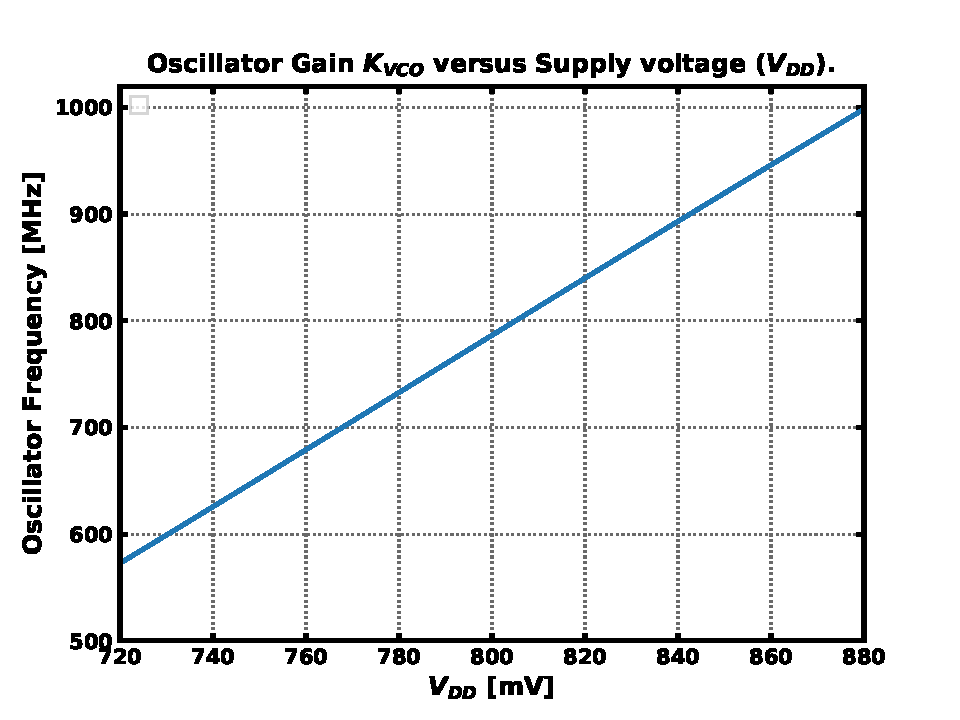
\includegraphics[width=1\textwidth, angle=0]{./figs/results/osc_f_vs_vdd}
	        \caption{ }
	        \label{fig:osc_f_vs_vdd}
	    \end{subfigure}%
	    \begin{subfigure}{0.5\textwidth}
	        \centering
	        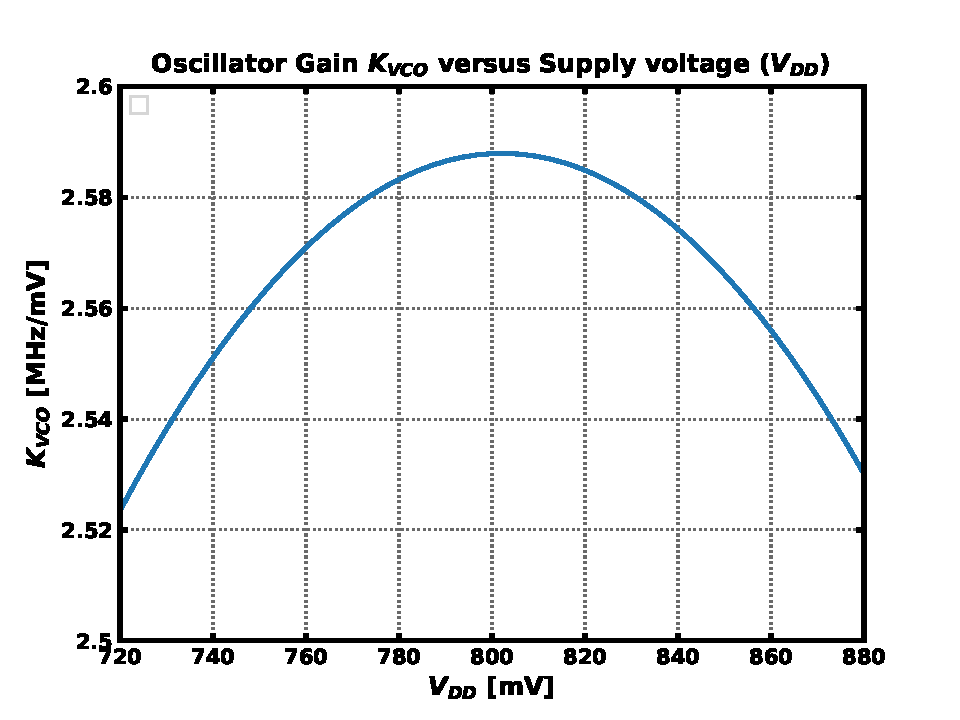
\includegraphics[width=1\textwidth, angle=0]{./figs/results/osc_f_gain_vs_vdd}
	        \caption{ }
	        \label{fig:osc_f_gain_vs_vdd}
	    \end{subfigure}
	    % \caption{x.}
	    \label{fig:osc_f_vdd}
	    \caption{Supply voltage versus ($\pm$ 10\% from 0.8V) \textbf{(a)} Oscillation Frequency, \textbf{(b)} VCO gain.}
	\end{figure} 

	\begin{figure}[htb!]
	    \centering
	    \begin{subfigure}{0.5\textwidth}
	        \centering
	        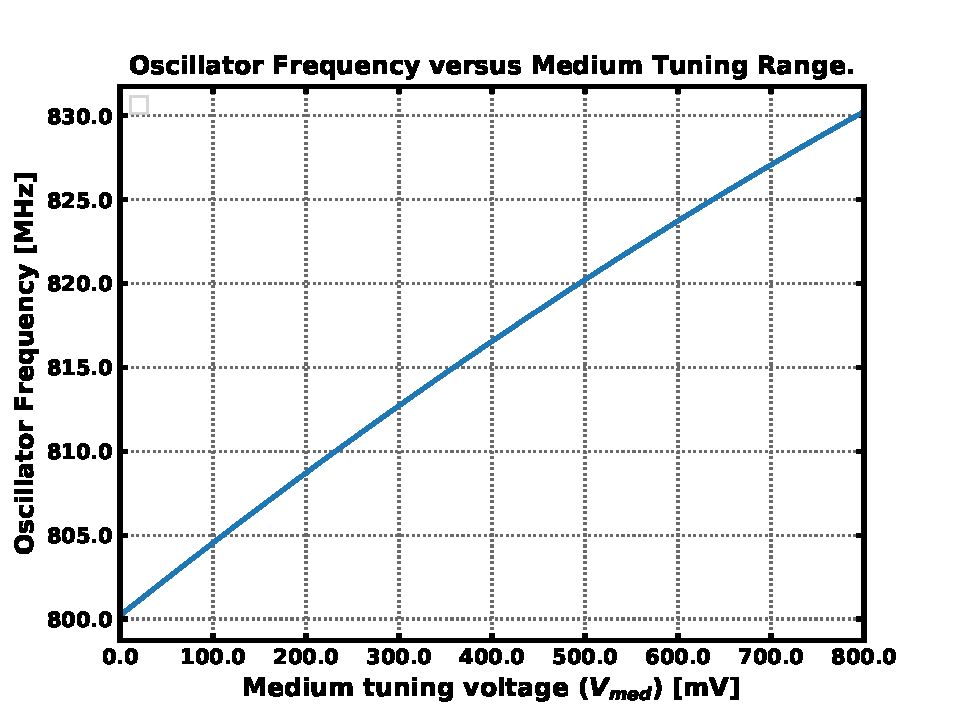
\includegraphics[width=1\textwidth, angle=0]{./figs/results/osc_f_vs_med}
	        \caption{ }
	        \label{fig:osc_f_vs_med}
	    \end{subfigure}%
	    \begin{subfigure}{0.5\textwidth}
	        \centering
	        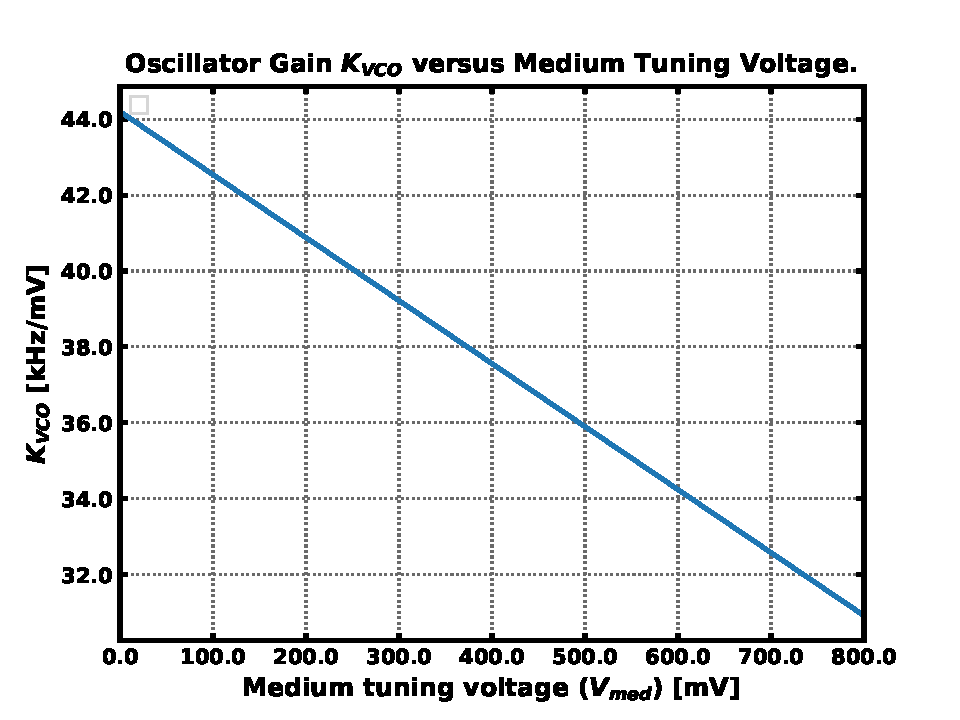
\includegraphics[width=1\textwidth, angle=0]{./figs/results/osc_f_gain_vs_med}
	        \caption{ }
	        \label{fig:osc_f_gain_vs_med}
	    \end{subfigure}
	    % \caption{x.}
	    \label{fig:osc_f_med_tune}
	    \caption{Medium tuning range versus \textbf{(a)} Oscillation Frequency, \textbf{(b)} VCO gain.}
	\end{figure} 


	\begin{figure}[htb!]
	    \centering
	    \begin{subfigure}{0.5\textwidth}
	        \centering
	        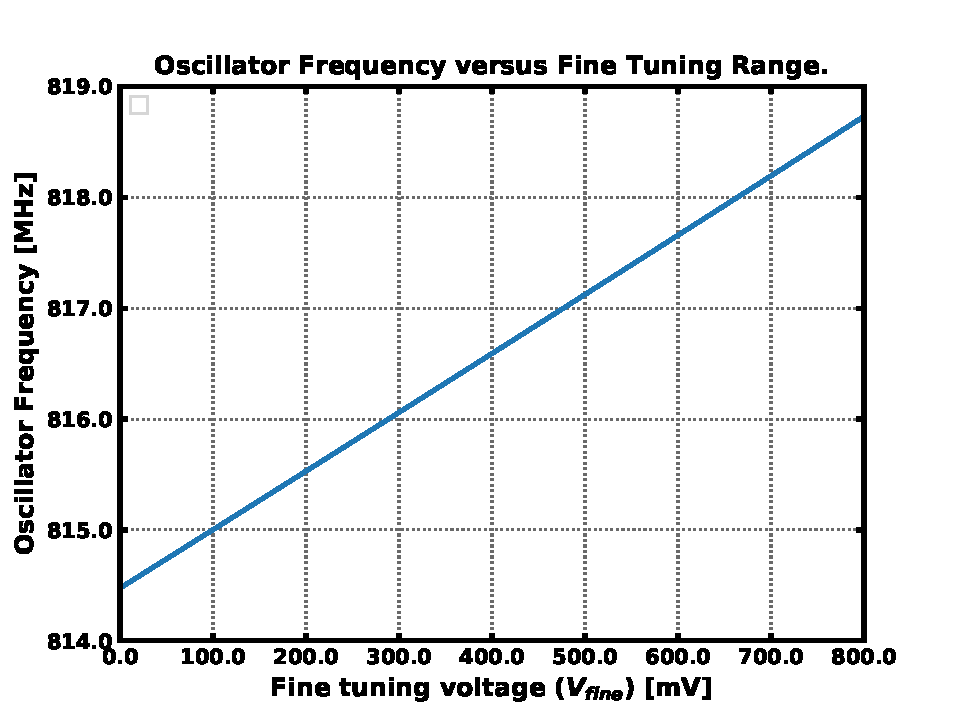
\includegraphics[width=1\textwidth, angle=0]{./figs/results/osc_f_vs_fine}
	        \caption{ }
	        \label{fig:osc_f_vs_fine}
	    \end{subfigure}%
	    \begin{subfigure}{0.5\textwidth}
	        \centering
	        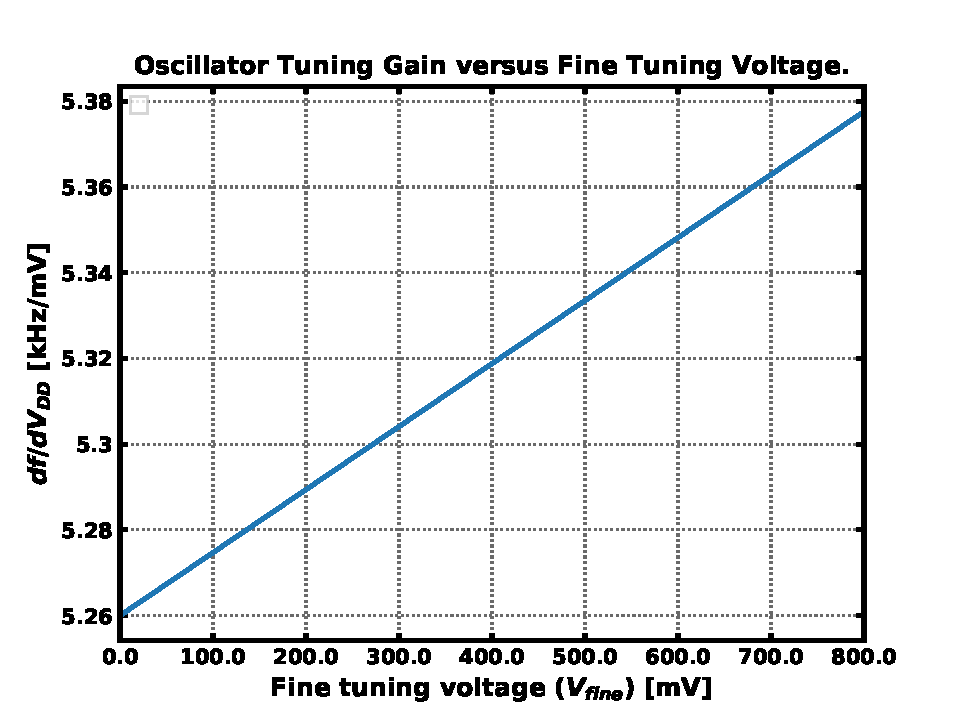
\includegraphics[width=1\textwidth, angle=0]{./figs/results/osc_f_gain_vs_fine}
	        \caption{ }
	        \label{fig:osc_f_gain_vs_fine}
	    \end{subfigure}
	    % \caption{x.}
	    \label{fig:osc_f_fine_tune}
	    \caption{Fine tuning range versus \textbf{(a)} Oscillation Frequency, \textbf{(b)} VCO gain.}
	\end{figure} 

{\color{white}.}\FloatBarrier
	\subsubsection{VCO Monte Carlo Simulation}

	\begin{figure}[htb!]
	    \centering
	    \begin{subfigure}{0.5\textwidth}
	        \centering
	        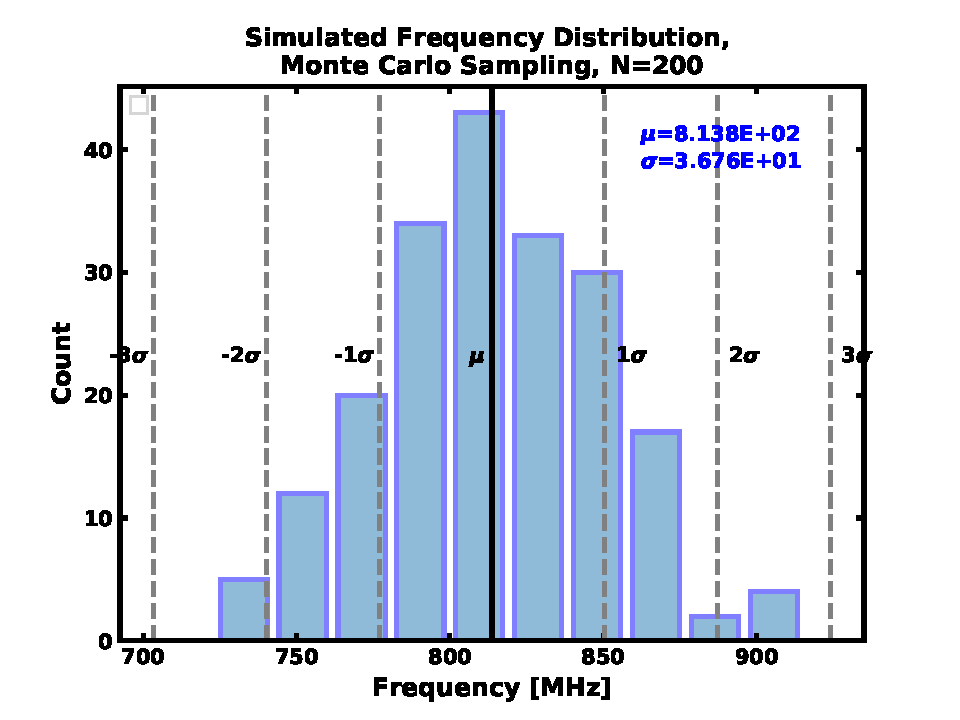
\includegraphics[width=1\textwidth, angle=0]{./figs/results/freq_hist_final}
	        \caption{ }
	        \label{fig:freq_variation}
	    \end{subfigure}%
	    \begin{subfigure}{0.5\textwidth}
	        \centering
	        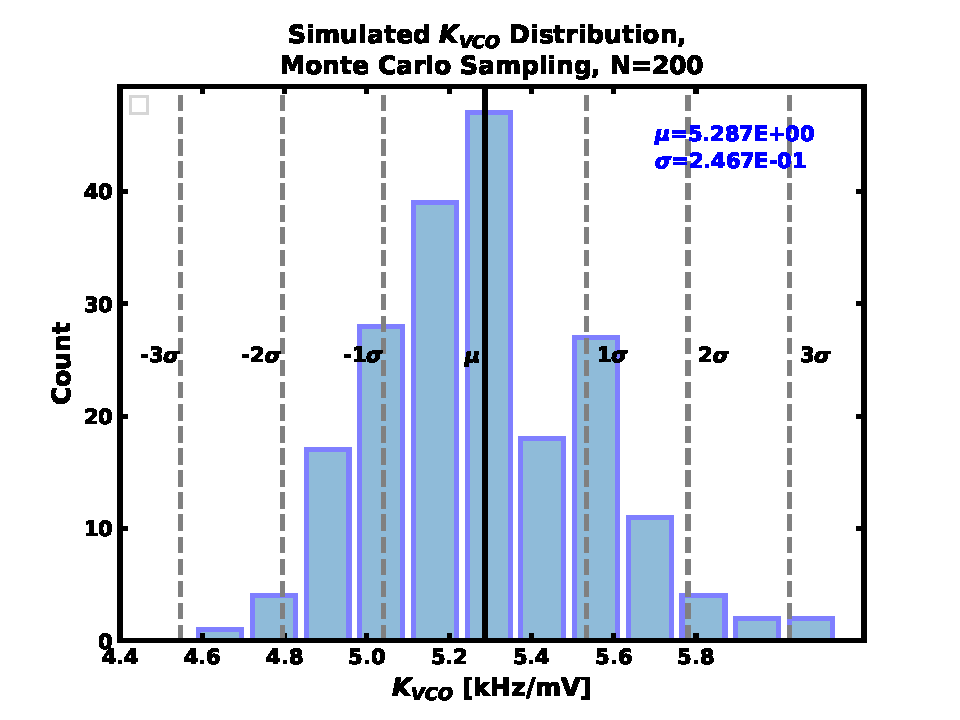
\includegraphics[width=1\textwidth, angle=0]{./figs/results/kvco_hist_final}
	        \caption{ }
	        \label{fig:kvco_variation}
	    \end{subfigure}
	    % \caption{x.}
	    \caption{\textbf{(a)} Variation of oscillator frequency from Monte-Carlo variation/mismatch simulation, \textbf{(b)} Variation of VCO fine tuning gain from Monte-Carlo variation/mismatch simulation.}
	    \label{fig:mc_sim_results}
	\end{figure} 
	\begin{table}[htb!]
		\def\arraystretch{1.5}		
		\setlength\arrayrulewidth{0.75pt}
		\setlength{\tabcolsep}{1em} % for the horizontal padding
		\begin{tabular}{|c|c|c|}
			\hline 
			\rule[-1ex]{0pt}{2.5ex} \cellcolor{gray!40}\textbf{Parameter} & \cellcolor{gray!40}\textbf{RMS Variance} & \cellcolor{gray!40}\textbf{Units}\\ 
			\hline 
			\rule[-1ex]{0pt}{2.5ex} \textbf{Frequency}&  36.762 \textbf{/} {\color{blue}4.50} &  MHz \textbf{/} {\color{blue}\%}  \\ 
			\hline 
			\rule[-1ex]{0pt}{2.5ex} \textbf{K$_\textnormal{\textbf{VCO, fine}}$} &  0.2467 \textbf{/} {\color{blue}4.67} &  MHz \textbf{/} {\color{blue}\%}  \\ 
			\hline 
		\end{tabular} 
		\caption{Ring oscillator Monte Carlo simulation extracted values.}
		\label{tab:mc_results}
	\end{table}

	{\color{white}.}
	\FloatBarrier\pagebreak
	\subsubsection{Waveforms}
			\begin{figure}[htb!]
			    \centering
			    \begin{subfigure}{0.5\textwidth}
			        \centering
			        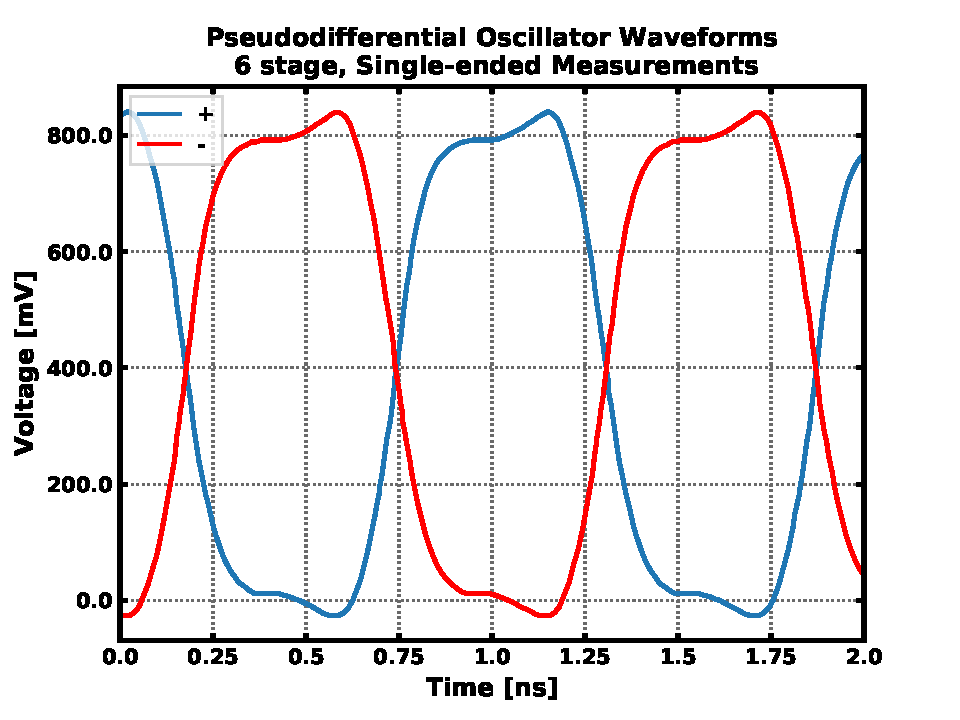
\includegraphics[width=1\textwidth, angle=0]{./figs/results/osc_se_waves}
			        \caption{ }
			        \label{fig:osc_se_waves}
			    \end{subfigure}%
			    \begin{subfigure}{0.5\textwidth}
			        \centering
			        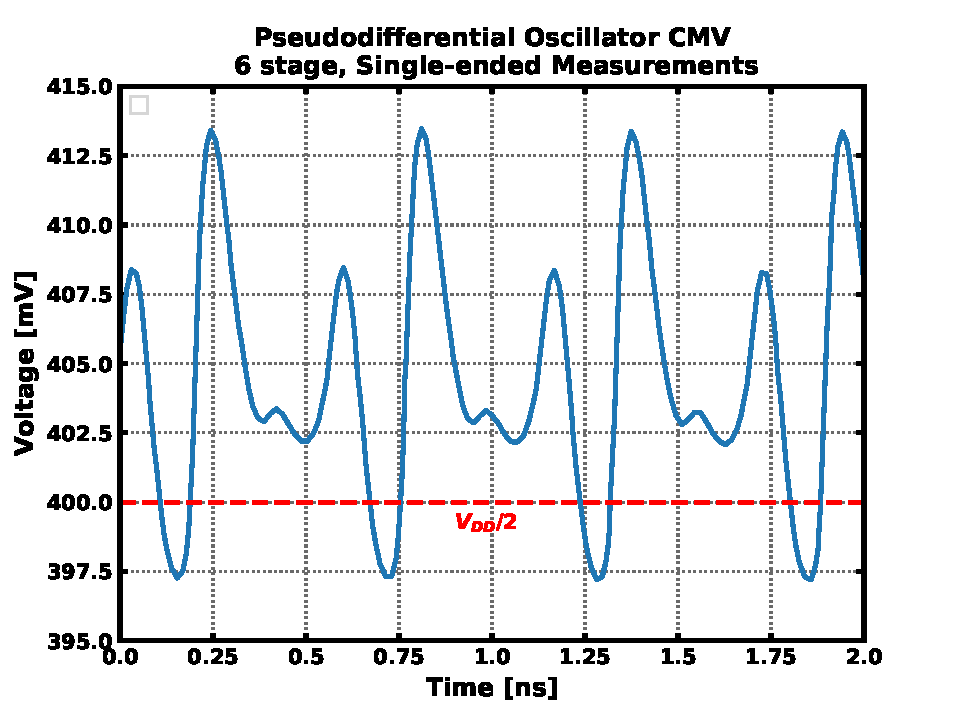
\includegraphics[width=1\textwidth, angle=0]{./figs/results/osc_cmv}
			        \caption{ }
			        \label{fig:osc_cmv}
			    \end{subfigure}
			    % \caption{x.}
			    \label{fig:osc_waves}
			    \caption{\textbf{(a)} Oscillator single-ended waveforms, \textbf{(b)} Oscillator common mode voltage waveform.}
			\end{figure} 
	\FloatBarrier
\FloatBarrier
\subsection{Oscillator Digitization}
\subsubsection{10b CDAC}\label{sec:res_cdac_10b}

	% \begin{figure}[htb!]
	%     \centering
	%     \begin{subfigure}{0.5\textwidth}
	%         \centering
	%         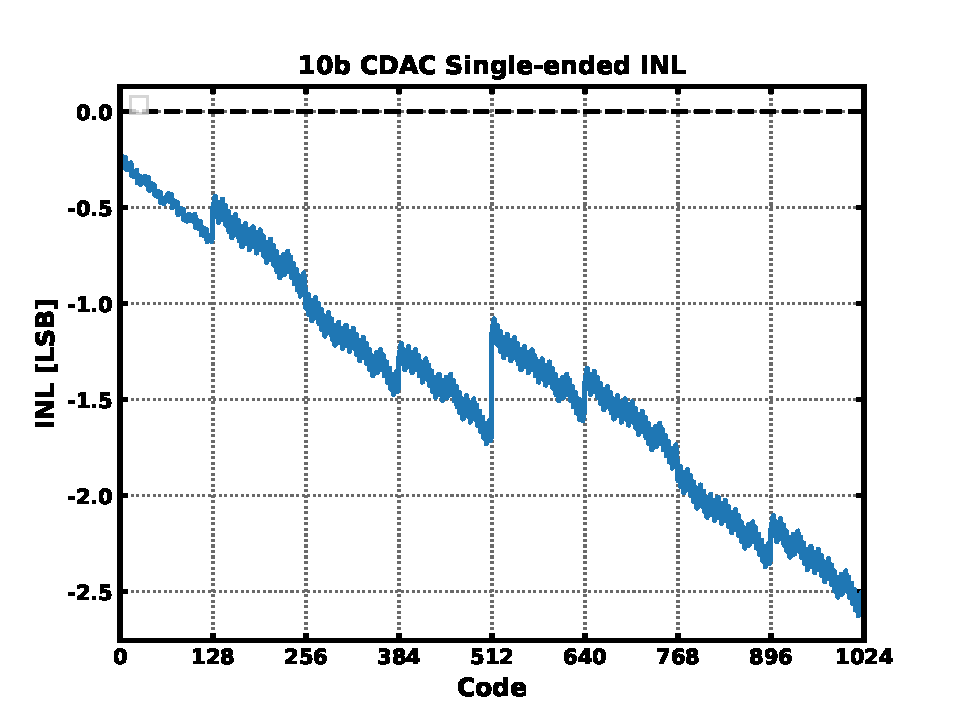
\includegraphics[width=1\textwidth, angle=0]{./figs/results/10b_cdac_se_inl}
	%         \caption{ }
	%         \label{fig:10b_cdac_se_inl}
	%     \end{subfigure}%
	%     \begin{subfigure}{0.5\textwidth}
	%         \centering
	%         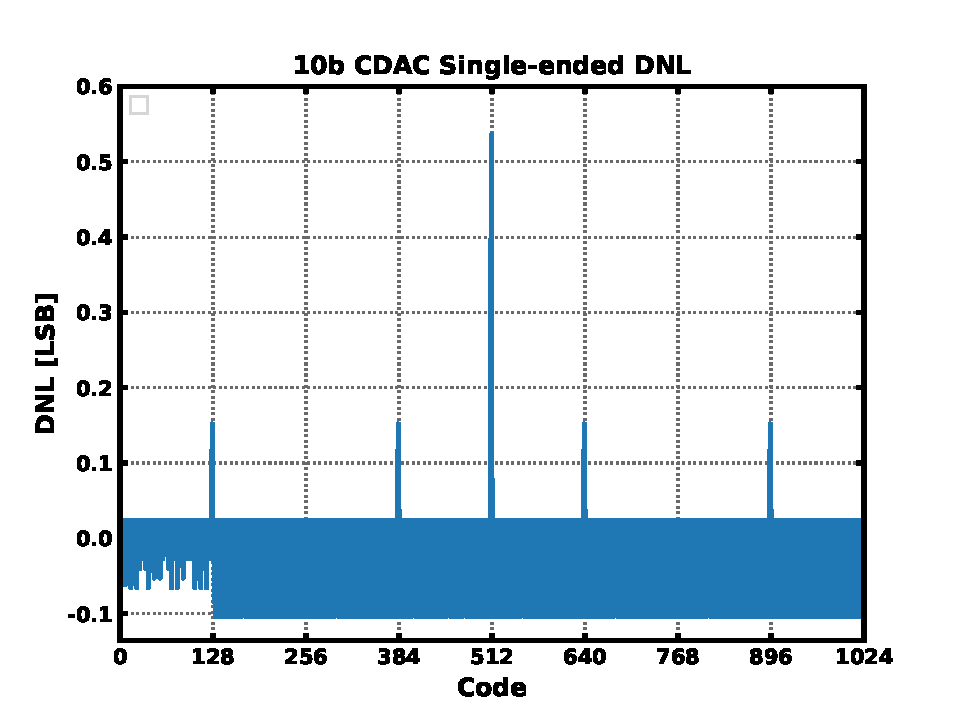
\includegraphics[width=1\textwidth, angle=0]{./figs/results/10b_cdac_se_dnl}
	%         \caption{ }
	%         \label{fig:10b_cdac_se_dnl}
	%     \end{subfigure}
	%     % \caption{x.}
	%     \label{fig:10b_cdac_se_nonlinearity}
	%     \caption{10b CDAC single-ended \textbf{(a)} Integral Nonlinearity, \textbf{(b)} Differential Nonlinearity.}
	% \end{figure} 



	\begin{figure}[htb!]
	    \centering
	    \begin{subfigure}{0.5\textwidth}
	        \centering
	        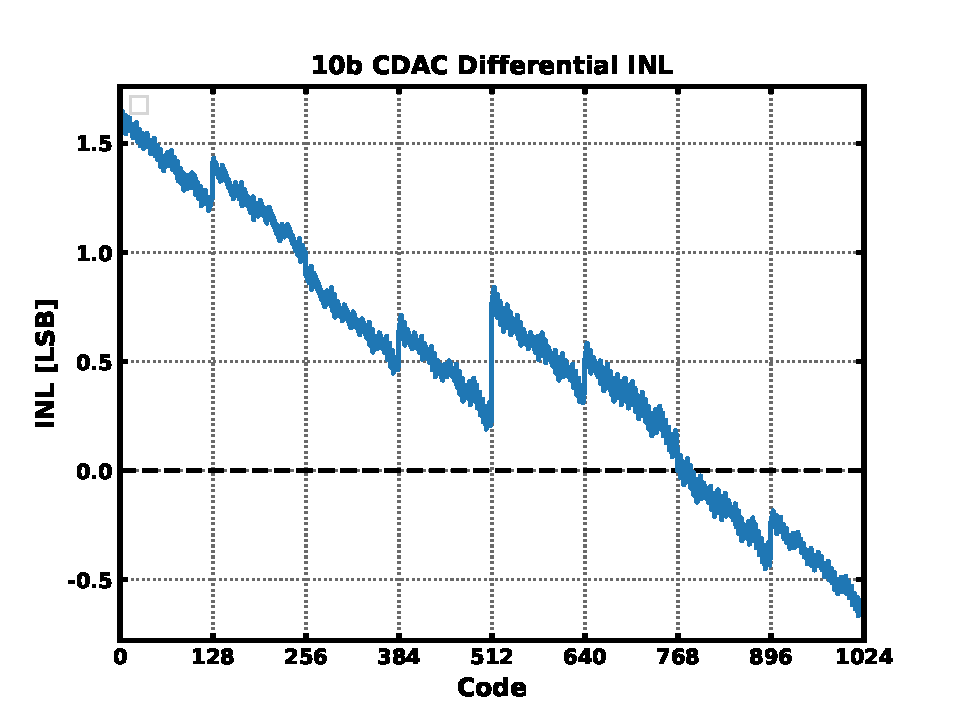
\includegraphics[width=1\textwidth, angle=0]{./figs/results/10b_cdac_diff_inl}
	        \caption{ }
	        \label{fig:10b_cdac_diff_inl}
	    \end{subfigure}%
	    \begin{subfigure}{0.5\textwidth}
	        \centering
	        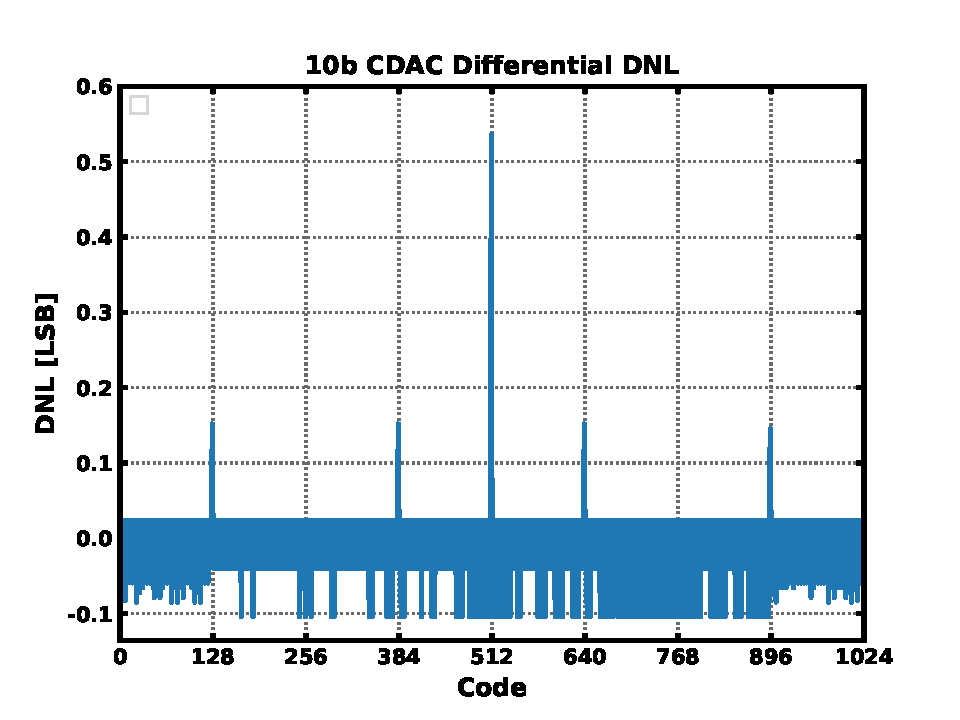
\includegraphics[width=1\textwidth, angle=0]{./figs/results/10b_cdac_diff_dnl}
	        \caption{ }
	        \label{fig:10b_cdac_diff_dnl}
	    \end{subfigure}
	    % \caption{x.}
	    \label{fig:10b_cdac_diff_nonlinearity}
	    \caption{Differential 10b CDAC \textbf{(a)} Integral Nonlinearity, \textbf{(b)} Differential Nonlinearity.}
	\end{figure} 

{\color{white}.}
\FloatBarrier\pagebreak
\subsubsection{3b CDAC}\label{sec:res_cdac_3b}

	\begin{figure}[htb!]
	    \centering
	    \begin{subfigure}{0.5\textwidth}
	        \centering
	        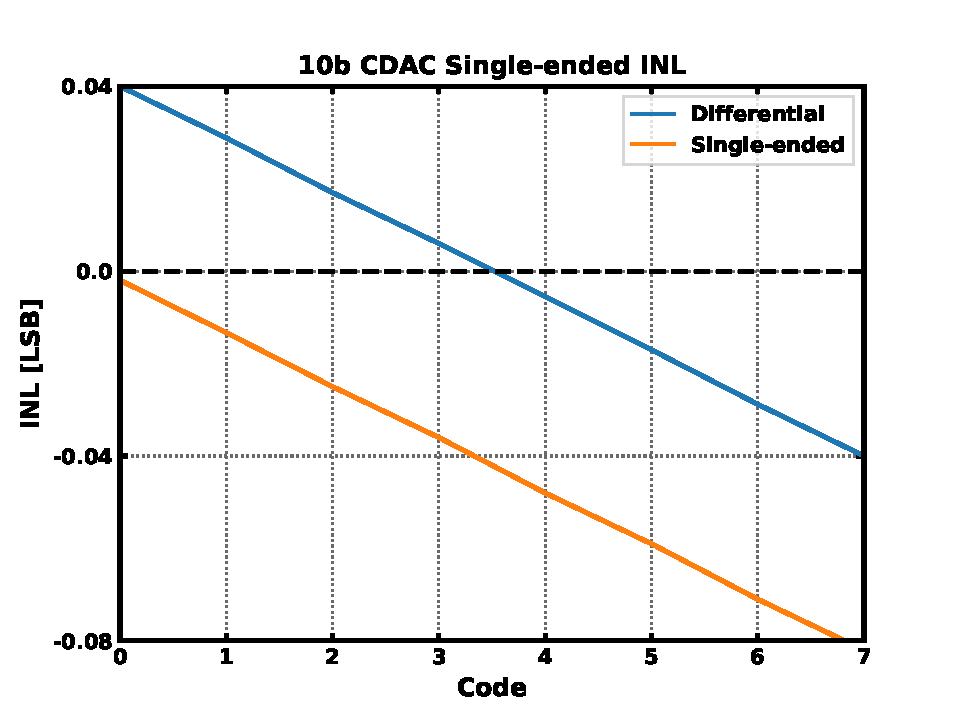
\includegraphics[width=1\textwidth, angle=0]{./figs/results/cdac_3b_inl}
	        \caption{ }
	        \label{fig:cdac_3b_inl}
	    \end{subfigure}%
	    \begin{subfigure}{0.5\textwidth}
	        \centering
	        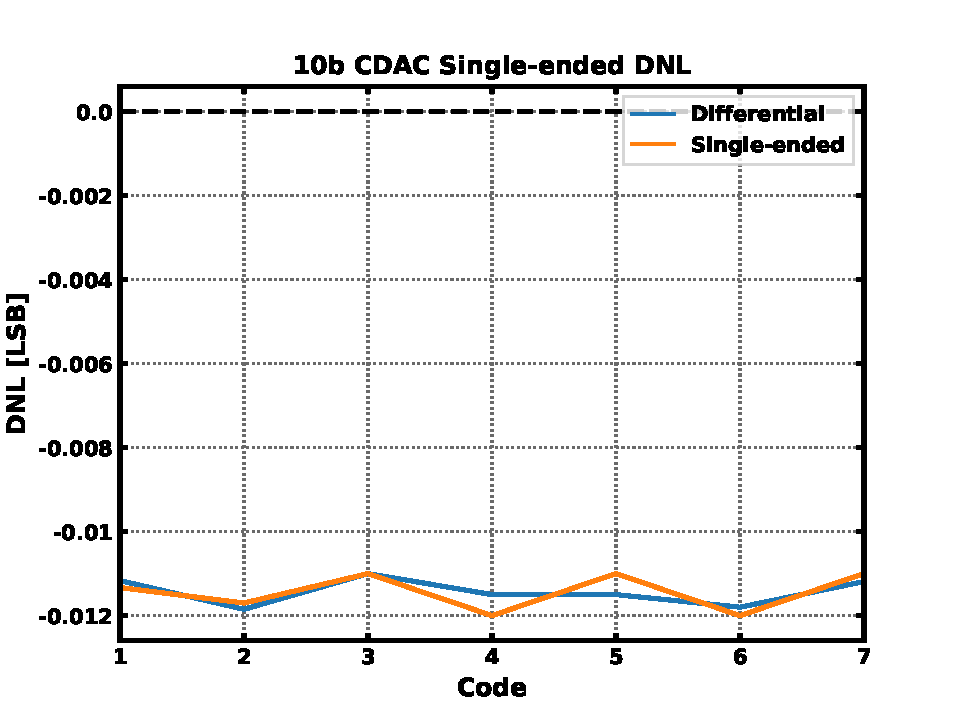
\includegraphics[width=1\textwidth, angle=0]{./figs/results/cdac_3b_dnl}
	        \caption{ }
	        \label{fig:cdac_3b_dnl}
	    \end{subfigure}
	    % \caption{x.}
	    \label{fig:3b_cdac_nonlinearity}
	    \caption{Differential  3b CDAC \textbf{(a)} Integral Nonlinearity, \textbf{(b)} Differential Nonlinearity.}
	\end{figure} 

\FloatBarrier
\subsubsection{DCO Gain}
\begin{table}[htb!]
	\def\arraystretch{1.5}		
	\setlength\arrayrulewidth{0.75pt}
	\setlength{\tabcolsep}{1em} % for the horizontal padding
	\begin{tabular}{|c|c|c|}
		\hline 
		\rule[-1ex]{0pt}{2.5ex} \cellcolor{gray!40}\textbf{Parameter} & \cellcolor{gray!40}\textbf{Value} & \cellcolor{gray!40}\textbf{Units}\\ 
		\hline 
		\rule[-1ex]{0pt}{2.5ex} \textbf{K$_\textnormal{\textbf{DCO, fine}}$} & 4.2 $\pm$ 0.53\tablefootnote{With $\pm 3 \sigma$ of process variation coverage.} & KHz/LSB \\ 
		\hline 
		% \rule[-1ex]{0pt}{2.5ex} $S_{0_{osc}}$ &  11885 &  rad$^2$/Hz  \\ 
		% \hline 
		\rule[-1ex]{0pt}{2.5ex} \textbf{K$_\textnormal{\textbf{DCO, med}}$} &  2.00 & KHz/LSB  \\ 
		\hline 
	\end{tabular} 
			\caption{DCO Gain values from final VCO gain and DAC results.}
			\label{tab:dco_gain}
\end{table}

\FloatBarrier
\subsection{Bang-bang Phase Detector}\label{sec:res_bbpd}
	\begin{figure}[htb!]
	    \centering
	    \begin{subfigure}{0.5\textwidth}
	        \centering
	        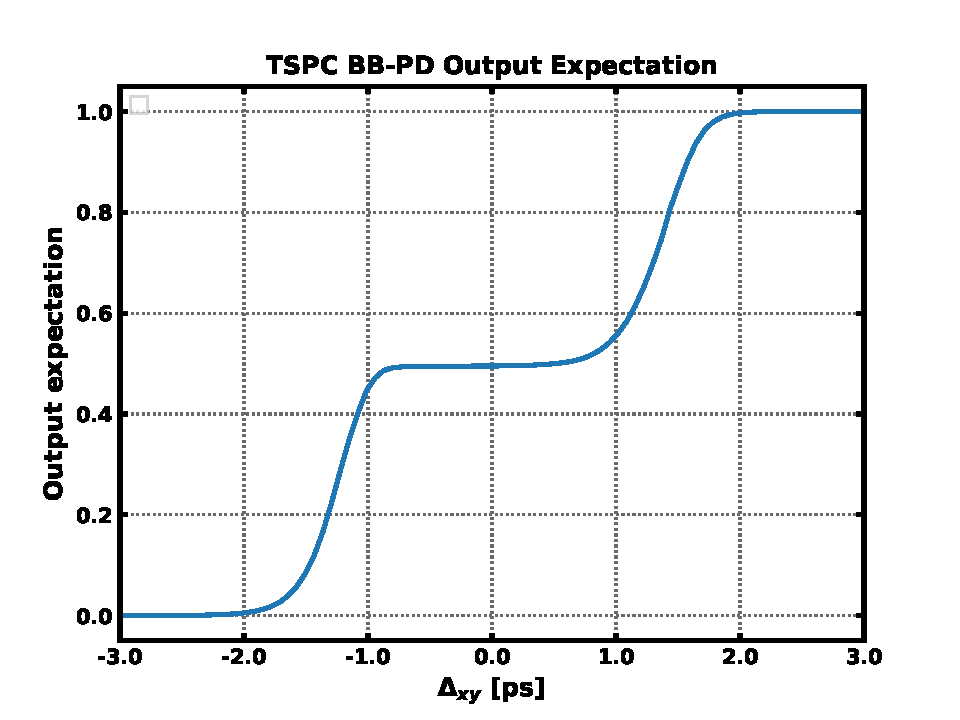
\includegraphics[width=1\textwidth, angle=0]{./figs/results/cdf}
	        \caption{ }
	        \label{fig:bbpd_cdf}
	    \end{subfigure}%
	    \begin{subfigure}{0.5\textwidth}
	        \centering
	        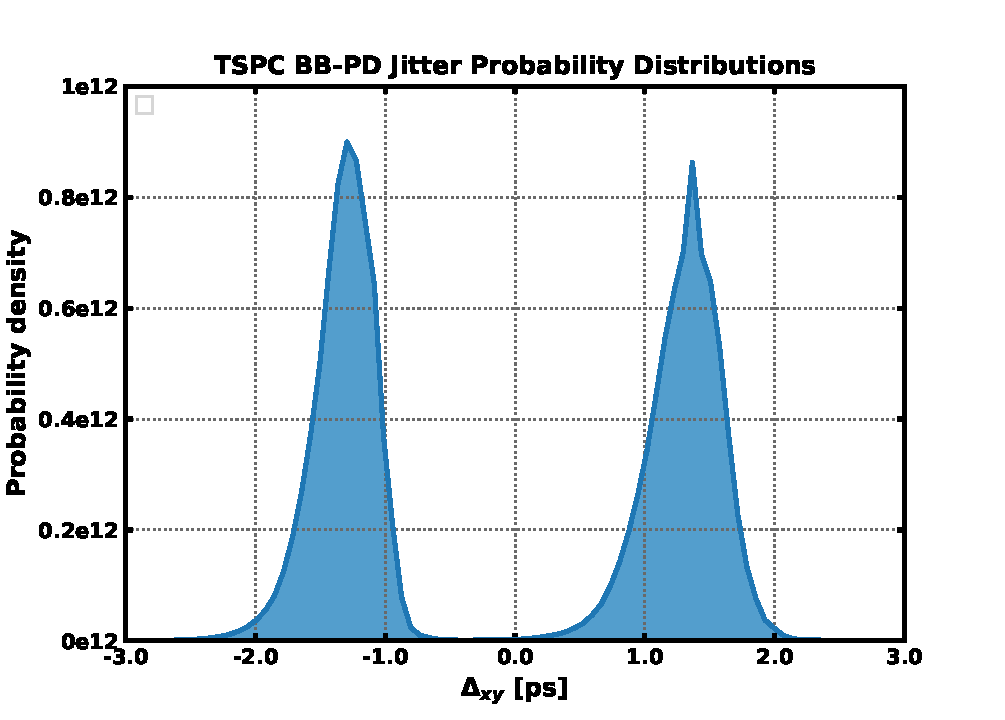
\includegraphics[width=1\textwidth, angle=0]{./figs/results/pdf}
	        \caption{ }
	        \label{fig:bbpd_pdf}
	    \end{subfigure}
	    % \caption{x.}
	    \label{fig:bbpd_jitter_dist}
	    \caption{BBPD extracted jitter \textbf{(a)} Cumulative Distribution Function, \textbf{(b)} Probability Distribution Function.}
	\end{figure} 
\FloatBarrier
\begin{table}[htb!]
	\def\arraystretch{1.5}		
	\setlength\arrayrulewidth{0.75pt}
	\setlength{\tabcolsep}{1em} % for the horizontal padding
	\begin{tabular}{|c|c|c|}
		\hline 
		\rule[-1ex]{0pt}{2.5ex} \cellcolor{gray!40}\textbf{Parameter} & \cellcolor{gray!40}\textbf{Value} & \cellcolor{gray!40}\textbf{Units}\\ 
		\hline 
		\rule[-1ex]{0pt}{2.5ex} \textbf{RMS Jitter} & 1.342 \tablefootnote{With noise simulated up to 20 GHz} & ps \\ 
		\hline 
	\end{tabular} 
			\caption{BBPD jitter extracted values.}
			\label{tab:bbpd_jitter}
\end{table}

\FloatBarrier\pagebreak
\subsection{Loop Filter }\label{sec:rec_lf}
	\subsubsection{Optimized Filter Parameters}
		\begin{table}[h!]
			\centering
			\def\arraystretch{1.5}		
			\setlength\arrayrulewidth{0.75pt}
			\setlength{\tabcolsep}{1em} % for the horizontal padding
			\begin{tabular}{|l|r|l|}
				\hline 
				\rule[-1ex]{0pt}{2.5ex} \cellcolor{gray!40}\textbf{Parameter} & \cellcolor{gray!40}\textbf{Value} & \cellcolor{gray!40}\textbf{Unit }\\ 
				\hline 
				\rule[-1ex]{0pt}{2.5ex} \textbf{$K$}  & $1.2008153\times12^{13}$ &  \\
				\hline 
				\rule[-1ex]{0pt}{2.5ex} \textbf{$K_i$}  & $3.8686562\times10^{7}$ &  \\
				\hline 
				\rule[-1ex]{0pt}{2.5ex} \textbf{$K_p$}  & $2.2328113\times10^{1}$ &  \\
				\hline 
				\rule[-1ex]{0pt}{2.5ex} \textbf{$f_z$}  & $2.7575807\times10^5$ & Hz\\
				\hline 
				\rule[-1ex]{0pt}{2.5ex} \textbf{$b_0$}  & $24.746023\times10^1$  &\\
				\hline 
				\rule[-1ex]{0pt}{2.5ex} \textbf{$b_1$}  & $-22.328113\times10^1$  & \\
				\hline 
				\rule[-1ex]{0pt}{2.5ex} Estimated bandwidth & $1.369080$ & MHz \\
				\hline 
				\rule[-1ex]{0pt}{2.5ex} Estimated RMS jitter & $13.5851$ & ps \\
				\hline 
			\end{tabular} 
			% \caption{Assigned specifications for branch line hybrid design.}
			% \label{asgn_specs}
			\caption{PLL parameters determined from filter design and optimization process for minimum phase noise with BBPD.}
			\label{filter_params_bbpd_low_noise}
		\end{table}   
		\subsubsection{Digital Filter Implementation Parameters}
		\begin{table}[h!]
			\centering
			\def\arraystretch{1.5}		
			\setlength\arrayrulewidth{0.75pt}
			\setlength{\tabcolsep}{1em} % for the horizontal padding
			\begin{tabular}{|l|r|r|l|}
				\hline 
				\rule[-1ex]{0pt}{2.5ex} \cellcolor{gray!40}\textbf{Parameter} & \cellcolor{gray!40}\textbf{Value} & \cellcolor{gray!40}\textbf{Value (digital) } & \cellcolor{gray!40}\textbf{Value Error}\\ 
				\hline 
				\rule[-1ex]{0pt}{2.5ex} Sign bits & 1 & & \\ 
				\hline 
				\rule[-1ex]{0pt}{2.5ex} Integer bits & 5 & & \\ 
				\hline 
				\rule[-1ex]{0pt}{2.5ex} Fractional bits & 8 & & \\ 
				\hline 
				\rule[-1ex]{0pt}{2.5ex} Total dataword bits & 14 & & \\ 
				\hline 
				\rule[-1ex]{0pt}{2.5ex} \textbf{$b_0$}  & $2.474609375\times10^1$ & \texttt{0b01100010111111}  & $+6.9880465\times10^{-5}$\\ 
				\hline 
				\rule[-1ex]{0pt}{2.5ex} \textbf{$b_1$}  & $-2.2328125\times10^1$ & \texttt{0b10100110101100}  & $-1.1305756\times10^{-5}$\\
				\hline 

			\end{tabular} 
			% \caption{Assigned specifications for branch line hybrid design.}
			% \label{asgn_specs}
			\caption{Loop filter digitized coefficients.}
			\label{dig_filter_params_fast}
		\end{table}  

{\color{white}.}
\FloatBarrier\pagebreak
\subsection{Logic}

		\begin{table}[htb!]
			\centering
			\def\arraystretch{1.5}		
			\setlength\arrayrulewidth{0.75pt}
			\setlength{\tabcolsep}{1em} % for the horizontal padding
			\begin{tabular}{|c|c|c|c|}
				\hline 
				\rule[-1ex]{0pt}{2.5ex} \cellcolor{gray!40}\textbf{Component} & \cellcolor{gray!40}\textbf{Count } & \cellcolor{gray!40}\textbf{Area [$\mu$m$^2$]}& \cellcolor{gray!40}\textbf{Area (\% total)}\\ 
				\hline 
				\rule[-1ex]{0pt}{2.5ex} \textbf{Sequential (DFF)} &  39 & 57.1 & 31.9 \\ 
				\hline 
				\rule[-1ex]{0pt}{2.5ex} \textbf{Inverter} & 29 & 3.86 & 2.2  \\ 
				\hline 
				\rule[-1ex]{0pt}{2.5ex} \textbf{Logic Gates} & 265 & 117.9 & 65.9  \\ 
				\hline 
				\rule[-1ex]{0pt}{2.5ex} \textbf{Total} & 333 & 178.9 & 100  \\ 
				\hline 
			\end{tabular} 
			\caption{Synthesized logic counts.}
			\label{tab:log_synth}
		\end{table}   

		\begin{table}[htb!]
			\centering
			\def\arraystretch{1.5}		
			\setlength\arrayrulewidth{0.75pt}
			\setlength{\tabcolsep}{1em} % for the horizontal padding
			\begin{tabular}{|c|c|c|c|}
				\hline 
				\rule[-1ex]{0pt}{2.5ex} \cellcolor{gray!40}\textbf{Voltage} & \cellcolor{gray!40}\textbf{Corner} & \cellcolor{gray!40}\textbf{Temperature [C]}& \cellcolor{gray!40}\textbf{Power [$\mu$W]}\\ 
				\hline 
				\rule[-1ex]{0pt}{2.5ex} 0.59 & SS & 40 & 2.33 \\ 
				\hline 
				\rule[-1ex]{0pt}{2.5ex} 0.59 & TT & 40 & 2.51  \\ 
				\hline 
				\rule[-1ex]{0pt}{2.5ex} 0.65 & TT & 25 & 12.1  \\ 
				\hline 
			\end{tabular} 
			\caption{Power consumption.}
			\label{tab:log_synth_power}
		\end{table}   

% \FloatBarrier\subsection{Synchronous counter}
% Power consumption
\FloatBarrier
{\color{white}.}